\documentclass[aspectratio=169]{beamer}
\usetheme[block=fill]{metropolis}
\usepackage{tikz}
\usetikzlibrary{shapes.geometric, arrows.meta, positioning, calc}

\title{Building a Reproducible Scholarly Search Toolkit}
\subtitle{Episode 10: Query Lexing \& Translation}
\author{Scholar Search Kit}
\date{}

\begin{document}

\begin{frame}[plain]
  \titlepage
\end{frame}

\begin{frame}{Episode Goal}
  \begin{alertblock}{The Goal}
    Build a Lexer that breaks a boolean string (\texttt{AI AND Health}) into tokens, and a Translator that maps those tokens to provider-specific syntax.
  \end{alertblock}
  \vspace{0.5cm}
  If the user writes \texttt{A AND B}, Semantic Scholar requires \texttt{A + B}, while Crossref might ignore it. We cannot let provider syntax dictate the user's research instrument.
\end{frame}

\begin{frame}{The Parsing Pipeline}
  \begin{center}
  \resizebox{0.8\linewidth}{!}{
  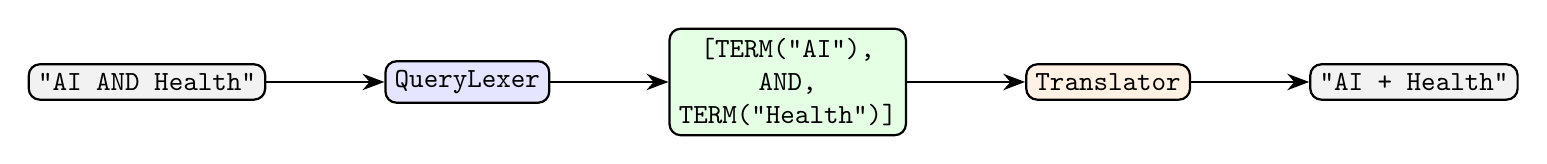
\begin{tikzpicture}[
      node distance=1cm and 1.5cm,
      string/.style={rectangle, draw, thick, rounded corners, fill=black!5, align=center},
      lexer/.style={rectangle, draw, thick, rounded corners, minimum width=2cm, fill=blue!10, align=center},
      tokens/.style={rectangle, draw, thick, rounded corners, fill=green!10, align=center},
      trans/.style={rectangle, draw, thick, rounded corners, minimum width=2cm, fill=orange!10, align=center},
      arrow/.style={-{Stealth[scale=1.2]}, thick}
    ]
    
    \node[string] (raw) {\texttt{"AI AND Health"}};
    \node[lexer, right=of raw] (lex) {\texttt{QueryLexer}};
    \node[tokens, right=of lex] (tok) {\texttt{[TERM("AI"),}\\\texttt{AND,}\\\texttt{TERM("Health")]}};
    \node[trans, right=of tok] (tran) {\texttt{Translator}};
    \node[string, right=of tran] (out) {\texttt{"AI + Health"}};
    
    \draw[arrow] (raw) -- (lex);
    \draw[arrow] (lex) -- (tok);
    \draw[arrow] (tok) -- (tran);
    \draw[arrow] (tran) -- (out);
  \end{tikzpicture}
  }
  \end{center}
\end{frame}

\begin{frame}{Implementation: `QueryLexer`}
  \begin{block}{Tokenization}
    We read the string character by character and emit a list of \texttt{QueryToken} objects.
  \end{block}
  
  \begin{itemize}
      \item \texttt{TokenType}: \texttt{TERM}, \texttt{AND}, \texttt{OR}, \texttt{NOT}, \texttt{LPAREN}, \texttt{RPAREN}.
      \item Handles quotes: \texttt{"Machine Learning"} is parsed as a single \texttt{TERM}.
  \end{itemize}
\end{frame}

\begin{frame}{Implementation: Translators}
  \begin{block}{The \texttt{QueryTranslator} Protocol}
    Each Provider will supply its own Translator to map tokens into its native format.
  \end{block}
  
  \begin{itemize}
      \item \texttt{SimpleQueryTranslator}: Strips all operators and just returns \texttt{AI Health} (for dumb APIs).
      \item \texttt{BooleanQueryTranslator}: Maps \texttt{AND} $\rightarrow$ \texttt{+}, \texttt{OR} $\rightarrow$ \texttt{|} (for Semantic Scholar).
  \end{itemize}
\end{frame}

\begin{frame}{Verification}
  \begin{alertblock}{Success Criteria}
    \begin{itemize}
        \item \texttt{"AI" AND (Health OR Medical)} parses to 7 distinct tokens.
        \item Translators correctly format complex nested tokens into provider-specific strings.
    \end{itemize}
  \end{alertblock}
\end{frame}

\end{document}
